The method of Convolutional Nerual Networks requires multiple layers in the process of trianing.
In a big picture, the layers could be divided into three layers: input, hidden, and output layers.
The input layer receives input, data such as matrices, and output layer produces the result values produced
by the model. Result values are N by the number of unique characters matrix that each vector contains the
probability of input to be the character of the corresponding index numbers. The layers are implemented while
utilizing the Tensorflow python package.
\newline
\newline
\indent
The hidden are further divided into three layers: Convolution, Flattening, and Fully Connected layers.
For this project, there are three convolution layers, one flattening layer, and two fully connected layers.
    \begin{figure}
        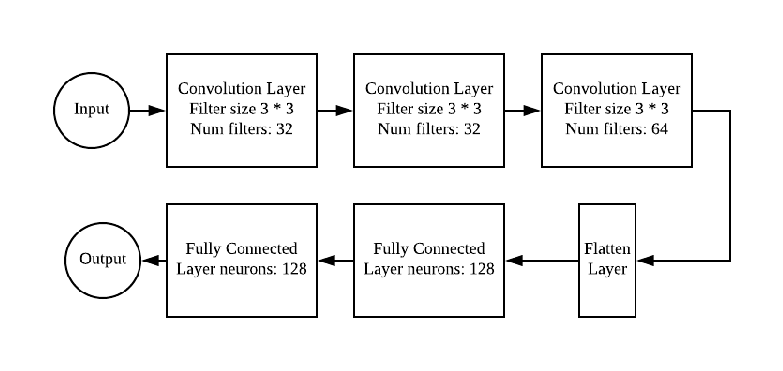
\includegraphics[width=\textwidth, scale=0.25]{flow.eps}
        \caption{Flow chart of training (convolutional neural netwokrs).\cite{sachan_2017}} \label{Figure1}
    \end{figure}

\subsubsection{Convolution Layer} is filtering layer.
Convolution layer applies filter to find patterns in the input image. The size of the filter is three by three matrices. The values
in the matrices are initially random numbers, which are weights. Also, biases are initially randomized.
However, this values will be updated in the back propagation
stage.
\newline
\newline
\indent
The number of filters are 32 in first two convolution layers and 64 in the last layer. Then, the filters with
weights will be applied to the input image and biases will be added after convolution phase. After filtering the
image and added biases, this layer will pool the max values in each filters. Finally, outputs from the pooling
function will be fed to the Relu function.
\newline
\newline
\indent
To be more specific, filtering a RGB image, size of 20 by 20 by three, with three by three filter and max pooling
function will create a matrix size of 18 by 18 by three. The matrix will be padded with zeros to reserve the original input
size. This output will be fed into the Relu function to remove negative values.

\subsubsection{Flattening Layer}
is reshaping outputs from convolution layers before feeding into fully connected layer. Simply,
this layer "use the reshape operation to create a single dimensional tensor."\cite{sachan_2017}


\subsubsection{Fully Connected Layer}
is defined to "receive input from all the neurons in the previous layer"\cite{sachan_2017} by applying
weights and biases to the input vectors. Initially, weights and biases are randomly chosen. However, this
will be adjusted during the back propagation process. After matrix multiplication, again, the reulu function
will be applied to remove negative values. Then the result outputs will be the probability of each tensor being
a prediction.
\newline
\newline
\indent
After inputs going through the layers, the model optimize the randomly initialized weights and biases. This process is called
\textbf{back propagation}.
From the output tensor from the last fully connected layer, this model utilizez the soft max function to find
the highest probabilities of the result. Then, it compares the predicted labels to the actual character label.
Based on the result of the prediction, the model calcualtes the cost by utilizing the cross entropy function and the
average of its result. Finally, this model "uses AdamOptimizer for gradient calculation and weight optimization."\cite{sachan_2017}
This model tries this method to minimize the cost with a learning rate of 0.0001.
